\documentclass{beamer}
\usepackage{amsmath, amssymb, amsthm, mathtools}
\usepackage{subfigure}
\usepackage{graphicx}
\usepackage{caption}
\usepackage{cancel}
% \usepackage{subcaption}

\newcommand{\bs}[1]{\boldsymbol{#1}}
\newcommand{\norm}[1]{\left\| #1 \right\|}
\newcommand{\snorm}[1]{\left| #1 \right|}
\newcommand{\LRp}[1]{\left( #1 \right)}
\newcommand{\LRs}[1]{\left[ #1 \right]}
\newcommand{\LRc}[1]{\left\{ #1 \right\}}
\newcommand{\Grad}{\ensuremath{\nabla}}
\newcommand{\Div}{\ensuremath{\nabla\cdot}}
\newcommand{\bfn}{\mbox{\boldmath $n$}}
\newcommand{\bfH}{\mbox{\boldmath $H$}}
\newcommand{\HdivK}{\bfH(\text{div},K)}
\newcommand{\HOneK}{H^{-1}(K)}
\newcommand{\HOneOmegah}{H^{-1}(\Omega_h)}
\newcommand{\HdivOmegah}{\bfH(\text{div},\Omega_h)}
\newcommand{\vdeltau}{v_{\delta\bs u_h}}
\newcommand{\taudeltau}{\btau_{\delta\bs u_h}}
\newcommand{\ip}[1]{\left\langle #1 \right\rangle}
\newcommand{\pd}[2]{\frac{\partial#1}{\partial#2}}
\newcommand{\pdd}[3]{\frac{\partial^2#1}{\partial#2\partial#3}}

\def\arr#1#2#3#4{\left[
\begin{array}{cc}
#1 & #2\\
#3 & #4\\
\end{array}
\right]}
\def\vecttwo#1#2{\left[
\begin{array}{c}
#1\\
#2\\
\end{array}
\right]}
\def\vectthree#1#2#3{\left[
\begin{array}{c}
#1\\
#2\\
#3\\
\end{array}
\right]}

\renewcommand{\arraystretch}{2.0}

\def\etal{{\it et al.~}}

\usetheme[secheader]{pecostalk}

\author[Truman E. Ellis]{Truman E. Ellis}
\title[Intro to LES]{Introduction to Large Eddy Simulation}
\institute{Institute for Computational and Engineering Sciences\\
The University of Texas at Austin}

\begin{document}

\begin{frame}
\titlepage
\end{frame}

\begin{frame}\frametitle{Filtered Navier-Stokes}
For filter kernel $G$,
\[
\overline{u}(x)=\int_\Omega G(x,x')u(x')dx'
\]
Filtering the incompressible Navier-Stokes equations:
\[
\pd{\overline{u_i}}{t}=-\overline{\pd{u_iu_j}{x_j}}-\overline{\pd{p}{x_i}}
+\nu\overline{\pdd{u_i}{x_j}{x_j}}
\]
If $G(x,x')=G(x-x')$, we can commute differentiation and filtering
\[
\pd{\overline{u_i}}{t}=-\pd{\overline{u_iu_j}}{x_j}-\pd{\overline{p}}{x_i}
+\nu\pdd{\overline{u_i}}{x_j}{x_j}
\]
Identify ``sub-grid stress'' analogous to Reynolds stress,
\[
\tau_{ij}=\overline{u_iu_j}-\bar{u_i}\bar{u_j}
\]
\end{frame}

\begin{frame}\frametitle{Common Filters}
Explicit Filters:
\begin{itemize}
\item Fourier cut-off filter
\[
\hat G(k) = \begin{cases}
1 & |k| < k_c \\
0 & |k| > k_c \\
\end{cases}
\]
Filter width $\Delta=\pi/k_c$.
\item Top-hat filter
\[
G(x) = \begin{cases}
1/\Delta & |x| < \Delta/2\\
0 & |x| > \Delta/2
\end{cases}
\]
\item Gaussian filter
\[
G(x)=\frac{e^{-x^2/2\Delta^2}}{\Delta\sqrt{2\pi}}
\]
\end{itemize}
Implicit Filters:
\begin{itemize}
\item The numerical method is the filter -- very common, but suspect
\item Define your filter as some projection of the Navier-Stokes solution onto
some finite dimensional function space
\end{itemize}
\end{frame}

\begin{frame}\frametitle{The Closure Problem}
\begin{block}{Filtered Navier-Stokes}
\[
\pd{\overline{u_i}}{t}+\pd{\bar{u_i}\bar{u_j}}{x_j}=-\pd{\overline{p}}{x_i}
+\nu\pdd{\overline{u_i}}{x_j}{x_j}-\pd{\tau_{ij}}{x_j}
\]
\end{block}
\begin{columns}[c]
\begin{column}{0.6\textwidth}
\begin{itemize}
\item Smaller scales can be modeled as isotropic homogeneous
\item Homogeneous isotropic turbulence is \textbf{much} easier to model
\item Primarily need to capture energy cascade effect with extra dissipation
\item Smagorinsky model
\[
\tau_{ij}=-(C_s\Delta)^2(2\overline{S}_{lm}\overline{S}_{lm})^{1/2}\overline{S}_{ij}
+\frac{1}{3}\tau_{kk}\delta_{ij}
\]
\end{itemize}
\end{column}
\begin{column}{0.4\textwidth}
\begin{figure}[t]
	\begin{center}
		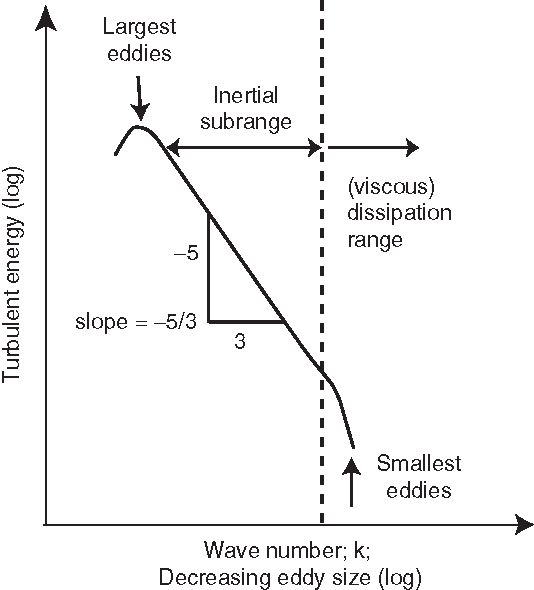
\includegraphics[width=\textwidth]{spectrum.png}
	\end{center}
\end{figure}
\end{column}
\end{columns}
\end{frame}

\begin{frame}\frametitle{The Dynamic Model}
Let $C=\sqrt{2}C_s^2$, then Germano's identity gives a process by which to
solve for $C$. Least squares solution gives
\[
C=\frac{\mathcal{L}_{ij}M_{ij}}{M_{kl}M_{kl}}
\]
where 
\[
M_{ij}=\Delta^2\LRp{\widetilde{|\overline{S}|\overline{S}_{ij}}-\alpha^2|\tilde{\overline S}|\tilde{\overline S}_{ij}}
\]
This fixed several longstanding issues with LES
\begin{itemize}
\item Adjustable constants are eliminated.
\item The model turns off (i.e. $C=0$) in well resolved or laminar regions.
\item The need for damping near the wall is eliminated.
\end{itemize}
\end{frame}

\begin{frame}\frametitle{Outstanding Problems -- Wall Modeling}
Near the wall, the ``large'' dynamicly important scales of turbulence are
actually quite small. Thus, to resolve the large scales, the LES must resolve
these small structures, and these structures get smaller relative to the
thickness of the shear layer as the Reynolds number increases. This makes LES
increasingly expensive with increasing Reynolds number. Wall modeling
techniques that do not require the near-wall structures to be resolved are
needed if LES is to be useful at high Reynolds number.
\end{frame}

\begin{frame}\frametitle{Outstanding Problems -- Numerical Errors}
It is common practice in LES for the filter width $\Delta$ to be the grid size
in the numerical simulation. The dynamic procedure uses the behavior of scales
between $\alpha\Delta$ and $\Delta$ is size to set the constants, but these
scales near the grid size have large numerical errors. Thus, the dynamic model
is working on data that is polluted by numerical errors. In fact, Ghosal
showed that even with high order numerical methods, the numerical truncation
errors can be much larger than the subgrid terms. There are three possible
solutions to this problem:
\begin{itemize}
\item Make $\Delta$ much larger than the grid size (expensive).
\item Use exceptionally accurate numerics, i.e. spectral methods (not
generally applicable).
\item Account for the numerical error in the formulation of the LES models (no
one knows how to do this).
\end{itemize}
\end{frame}

\begin{frame}\frametitle{Outstanding Problems -- Embedded laminar features}
In some flows, not everything is turbulent, and the features of the laminar
flow can be too small to resolve. Good examples of this are the separation
shear layers in the cross flow past a circular cylinder. These laminar
features cannot be resolved, but the models are not valid for them either.
\end{frame}

\begin{frame}\frametitle{Outstanding Problems -- What did you compute?}
In an LES, one does not compute the velocity field, rather one computes a
filtered velocity, and therefore one needs to be careful in interpreting the
results. For example, if one is interested in the statistical quantity
$\langle u^2\rangle$, one cannot determine this exactly from the LES. In the
LES, one can only determine $\LRa{\overline{u}^2}\neq\LRa{u^2}$, unless the
energy in the subgrid turbulence is negligible. In general one can expect to
estimate such statistical quantities as $\LRa{u_i(x+r)u_j(x)}$ accurately
provided $|r|\gg\Delta$. However, since the vorticity is strictly a
small-scale quantity (the subgrid contribution to enstrophy is not small), one
cannot expect to reproduce vorticity statistics in an LES.
\end{frame}

\begin{frame}\frametitle{Outstanding Problems -- Commutation Error}
Filters that are used in actual LES simulations are not generally homogeneous,
that is $G(x,x')\neq G(x-x')$, so that filtering no longer commutes with
differentiation. Then, most significantly,
\[
\overline{\pd{u_iu_j}{x_j}}\neq\pd{\overline{u_iu_j}}{x_j}\,,
\]
and the difference between these two terms is generally called the commutation
error. This commutation error plays an important role in the equations.
Suppose that a flow domain is divided into two regions, one in which the
filter scale $\Delta$ is larger than in the other region. If trubulence passes
from the small filter scale region to the large, then not all the scales of
the turbulence that could be represented in the finer region can be
represented in the coarser region. Therefore, some of the smaller scales must
be removed as the turbulence passes from one region to the other. When
turbulence is passing the the opposite direction, scales that were not
represented become representable, and must be added to the LES solution. 
\end{frame}

\begin{frame}\frametitle{Variational Multiscale LES}
\begin{itemize}
\item Use variational projections in place of the traditional filtered
equations
\item Focus on modeling the fine-scale equations
\item Avoids filters eliminates:
\begin{itemize}
\item Inhomogeneous non-commutative filters necessary for wall-bounded flows
\item Use of complex filtered quantities in compressible flows
\end{itemize}
\item Retains numerical consistency in the coarse-scale equations permitting
full rate-of-convergence
\item Newer approaches attempt to capture all scales consistently and to avoid use of eddy
viscosities altogether
\end{itemize}
\end{frame}

\end{document}
